\chapter{Introduction}
\label{ch:introduction}

\begin{tcolorbox}[colback=tumorcell!10, colframe=tumorcell!50, title=\textbf{The Stakes}]
\textit{"Every 90 minutes, someone dies from kidney cancer. Behind each statistic lies a patient, a family, a life interrupted. What if we could see the invisible war raging inside their bodies and learn to tip the balance toward healing?"}
\end{tcolorbox}

\section{When Cells Go Rogue: The Hidden Battlefield of Renal Cell Carcinoma}
\label{sec:intro_epidemiology}

Within the human kidney, normally a marvel of biological engineering that filters 50 gallons of blood daily, something goes terribly wrong for 400,000 people every year. A single cell---perhaps damaged by a cigarette's toxins, stressed by years of hypertension, or simply unlucky in the genetic lottery---breaks free from its programming. This rogue cell begins to multiply relentlessly, ignoring the body's desperate signals to stop.

This is renal cell carcinoma (RCC), and it represents far more than medical statistics. It's a molecular rebellion that unfolds in three-dimensional space, where every cubic millimeter tells a story of cellular warfare.

The numbers tell part of the tale: RCC claims the lives of roughly 175,000 people annually worldwide, making it the deadliest urological cancer \cite{santoni2024}. But numbers cannot capture what happens next---the intricate dance between rebel tumor cells and the immune system's desperate attempts to restore order.

\subsection{The Deadly Mathematics of Late Discovery}

Here's what makes RCC particularly insidious: it's a silent killer. Unlike other cancers that announce themselves with pain or obvious symptoms, RCC often grows undetected in the kidney's depths. The kidney, remarkably, can function normally even when half-consumed by tumor. By the time symptoms appear---blood in urine, flank pain, an abdominal mass---it's often too late.

The survival statistics paint a stark picture. Catch RCC early, confined to the kidney, and five-year survival rates climb to 75\%. But for the one-third of patients who present with metastatic disease, that number plummets to a devastating 15\% \cite{rini2019}. The difference between life and death often comes down to a matter of timing and detection---and increasingly, understanding the invisible war happening at the cellular scale.

Clear cell RCC (ccRCC) constitutes 70--80\% of all RCC cases and is characterized by mutations in the \emph{VHL} gene, which lead to constitutive activation of the hypoxia-inducible factor (HIF) pathway and consequent overexpression of vascular endothelial growth factor (VEGF). This molecular hallmark has made ccRCC a prototypical target for anti-angiogenic therapies, while its relatively high immunogenicity---evidenced by dense immune infiltrates and occasional spontaneous regressions---has positioned it as one of the tumors most responsive to immunotherapy \cite{pardoll2012}.

\section{Inside the Cellular Battlefield: Decoding the Tumor Microenvironment}
\label{sec:intro_tme}

Imagine shrinking down to the scale of a single cell and stepping into the tumor microenvironment. You'd find yourself in a landscape as complex and dynamic as any major city---but this is a city at war.

The tumor microenvironment isn't just tumor cells run amok. It's an entire ecosystem spanning hundreds of microns, where eighteen distinct cellular populations navigate a three-dimensional maze of blood vessels, navigate chemical gradients, and engage in life-or-death communication through molecular signals. Think of it as a microscopic metropolis where every resident plays a role in determining whether the patient lives or dies.

\subsection{The Cast of Cellular Characters}

Within this microscopic theater, each cell type has its own agenda:

\textbf{Tumor cells}---the villains of our story---don't just multiply blindly. Each carries its own unique genetic signature, a 16-gene molecular fingerprint that determines how aggressively it grows, whether it can hide from immune detection, and how it responds to treatment. Like criminals with different skill sets, some tumor cells specialize in rapid growth, others in immune evasion, still others in building blood supply networks.

\textbf{The immune system's army} arrives in waves. Cytotoxic T cells act as elite special forces, capable of precision strikes against tumor cells they recognize as foreign. But they need intelligence---provided by dendritic cells, the reconnaissance specialists who survey the battlefield, capture tumor fragments, and brief the T cells on their targets. Natural killer cells patrol as the first responders, attacking anything that looks suspicious.

Yet the tumor fights back with cunning. It recruits double agents---regulatory T cells and M2 macrophages---that sabotage immune responses from within. It hijacks the blood supply, commandeering vessels to feed its insatiable appetite for glucose. Most deviously, it learns to wear molecular disguises, expressing PD-L1 molecules that act like a "don't shoot" signal to approaching T cells.

\textbf{The metabolic supply lines} tell their own story. Blood vessels pump glucose into the battlefield like fuel trucks supplying an army. But tumor cells, following the Warburg effect, consume glucose at rates up to 200 times higher than normal cells, creating zones of metabolic starvation that cripple immune cell function.

\subsection{The Invisible War}

What makes this war particularly complex is that it's not a simple good-versus-evil narrative. The interactions are bidirectional, nonlinear, and often paradoxical. An immune cell that arrives to destroy tumor cells might instead be converted into a tumor-supporting ally. A blood vessel intended to nourish healthy tissue becomes a highway for tumor spread. A hormone meant to regulate normal physiology becomes a tumor's accomplice.

Understanding these dynamics isn't just an academic exercise. It's the key to understanding why some patients respond dramatically to immunotherapy while others don't---and why we desperately need new tools to peer into this cellular chaos and find patterns that could save lives.

\section{The Male-Female Divide: Why Sex Matters in Cancer's War}
\label{sec:intro_sex_differences}

Here's a medical mystery that has puzzled oncologists for decades: men are twice as likely to develop kidney cancer as women. At first glance, this might seem like just another statistic. But dig deeper, and you uncover a profound truth about human biology---our sex hormones aren't just about reproduction. They're powerful commanders in the immune system's war against cancer.

\begin{keyfinding}
The 2:1 male-to-female ratio in kidney cancer isn't just epidemiology---it's a biological signature pointing to sex hormones as master regulators of immune-tumor interactions, with direct implications for personalized treatment strategies.
\end{keyfinding}

\subsection{When Biology Becomes Destiny}

The numbers are stark and consistent across every population studied: male, 2:1 odds. Female, significantly better survival. This isn't coincidence---it's biology in action.

Traditional explanations point to lifestyle differences. Men smoke more, work in more hazardous environments, and generally engage in riskier behaviors. But these factors explain only part of the gap. The real story lies in the molecular messages coursing through our bloodstream---estrogen, testosterone, and progesterone---hormones that turn out to be master regulators of immune function.

\subsection{Estrogen: The Immune System's Double-Edged Sword}

Estrogen operates like a sophisticated immune system conductor, but its symphony changes dramatically depending on concentration. At moderate levels, estrogen acts as an immune enhancer, promoting the aggressive Th1 T cell responses that can eliminate tumor cells. It increases interferon-gamma production, boosts MHC molecule expression (the cellular equivalent of displaying a "wanted poster"), and enhances T cell killing capacity.

But here's where biology gets complex: at higher concentrations, estrogen flips the script. It shifts immune responses toward the gentler Th2 pathway, promotes the differentiation of regulatory T cells that suppress immune responses, and upregulates PD-1---the molecular brake pedal that tumors exploit to escape immune destruction \cite{conforti2018}.

\textbf{Testosterone tells a simpler, darker story.} Higher testosterone levels consistently suppress immune responses, reducing T cell proliferation and making immune evasion easier for tumors. This helps explain why men, with their higher testosterone burden, face worse kidney cancer outcomes.

\subsection{The ARON-1 Quest: Personalized Medicine Meets Sexual Biology}

These discoveries have sparked a revolutionary question: What if we could tailor cancer treatments based not just on tumor genetics, but on the patient's sex and hormonal profile?

Enter the ARON-1 clinical study \cite{santoni2024}---a groundbreaking investigation that asks whether the optimal immunotherapy approach depends on whether you're male or female. This isn't just medical curiosity; it's the future of personalized cancer care, where treatment protocols are designed around the unique biological landscape of each patient's hormonal and immune environment.

The computational model at the heart of this thesis was born from ARON-1's findings, designed to decode the complex interplay between sex hormones, immune responses, and treatment outcomes---and ultimately help clinicians choose the right therapy for the right patient at the right time.

\section{Why Virtual Tumors Matter: The Case for Computational Modeling}
\label{sec:intro_motivation}

Imagine if you could press pause on a patient's cancer, rewind the biological clock, and test thousands of different treatment combinations to find the one that works best. Imagine if you could peer into the microscopic chaos of the tumor microenvironment, watching immune cells hunt their targets, tracking how hormones shift the balance of power, and predicting treatment resistance before it happens.

\vspace{1em}

This isn't science fiction---it's computational biology. And for kidney cancer patients facing life-or-death treatment decisions, it might be the key to personalized therapy that saves lives.

\begin{keyinsight}
Computational modeling allows us to explore thousands of virtual treatment scenarios that would be impossible to test ethically in real patients, potentially revealing optimal therapy combinations years before traditional clinical trials could validate them.
\end{keyinsight}

\subsection{The Limits of Traditional Research}

Traditional cancer research faces three fundamental constraints that computational modeling can help overcome:

\vspace{1em}

\textbf{The Ethics Barrier.} You can't experiment on cancer patients. Clinical trials test one treatment protocol at a time, on carefully selected populations, under strictly controlled conditions. But what about the patient who doesn't fit the inclusion criteria? What about the combination therapy that might work but has never been tested? What about the treatment schedule that could be optimal but would take decades to validate?

\vspace{0.5em}

\textbf{The Time Barrier.} Cancer doesn't wait for research to catch up. A clinical trial takes 5-10 years from conception to results. During that time, thousands of patients with similar cancers face treatment decisions based on limited data from previous generations of trials.

\vspace{0.5em}

\textbf{The Complexity Barrier.} The human tumor microenvironment involves hundreds of cell types, thousands of molecular signals, and millions of possible interactions. Traditional experimental approaches excel at studying individual pathways but struggle to capture the emergent complexity that determines whether a patient lives or dies.

\begin{center}\rule{0.5\textwidth}{0.5pt}\end{center}

\subsection{The Promise of Virtual Patients}

Computational modeling offers a different approach---one that can complement and accelerate traditional research:

\begin{tcolorbox}[colback=immunecell!10, colframe=immunecell!50, title=\textbf{In Silico Experimentation}]
\textit{Virtual experiments that would be impossible in the real world.} Simulate thousands of virtual patients with different genetic profiles, hormone levels, and treatment regimens. Test combination therapies, explore dosing schedules, and identify biomarkers---all in hours rather than years. Each virtual patient becomes a hypothesis generator for future clinical validation.
\end{tcolorbox}

\textbf{Parameter Space Exploration.} The model becomes a high-dimensional map of treatment outcomes. Which biological variables matter most? How do sex hormones interact with immunotherapy response? Where are the tipping points between tumor control and immune escape? Computational exploration can guide experimental design and focus research efforts where they're most likely to yield insights.

\textbf{Treatment Optimization.} By coupling sophisticated simulations with machine learning algorithms, we can search for optimal treatment strategies tailored to individual patient profiles. The model becomes a virtual oncologist's assistant, exploring thousands of treatment permutations to find the most promising approach for each patient's unique biological landscape.

\textbf{Hypothesis Generation.} Perhaps most importantly, complex models generate unexpected insights---emergent behaviors that arise from the interaction of simple rules but wouldn't be obvious from studying individual components. These computational surprises often point toward new therapeutic targets or reveal hidden mechanisms of resistance.

\begin{figure}[H]
\centering
% Conceptual Overview Diagram for Chapter 1
\begin{tikzpicture}[scale=0.8, every node/.style={scale=0.8}]

% Define professional color palette
\definecolor{patient}{RGB}{67, 56, 202}       % Indigo
\definecolor{tumor}{RGB}{220,20,60}          % Crimson
\definecolor{immune}{RGB}{16, 185, 129}      % Emerald  
\definecolor{treatment}{RGB}{245, 158, 11}   % Amber
\definecolor{prediction}{RGB}{138,43,226}    % Purple
\definecolor{validation}{RGB}{249, 115, 22}  % Orange

% Patient input
\node[draw, rounded corners=3pt, fill=patient!20, text width=3cm, text centered, drop shadow] (patient) at (0,8) {
    \textbf{Patient Input}\\
    • Sex (M/F)\\
    • BMI\\
    • Tumor Volume\\
    • Mutation Profile
};

% Simulation layer
\node[draw, rounded corners=3pt, fill=immune!10, text width=12cm, text centered, minimum height=6cm, drop shadow] (simulation) at (6,5) {
    \textbf{Agent-Based Simulation}\\
    \vspace{0.3cm}
    \begin{minipage}{11cm}
        18 Agent Types • 3D Spatial Grid • Glucose Field\\
        MPI Parallel Execution • Repast4Py Framework
    \end{minipage}
};

% Tumor cells
\node[draw, circle, fill=tumor, text=white, drop shadow] (tumor1) at (3,6) {TC};
\node[draw, circle, fill=tumor, text=white, drop shadow] (tumor2) at (3.5,5.5) {TC};
\node[draw, circle, fill=tumor, text=white, drop shadow] (tumor3) at (2.5,5.5) {TC};

% Immune cells
\node[draw, circle, fill=immune, text=white, drop shadow] (tcell1) at (5,6.5) {CTL};
\node[draw, circle, fill=immune, text=white, drop shadow] (tcell2) at (5.5,6) {NK};
\node[draw, circle, fill=immune, text=white, drop shadow] (macro) at (4.5,5.5) {M1};
\node[draw, circle, fill=immune, text=white, drop shadow] (dc) at (6,5.5) {DC};

% Blood vessels
\draw[line width=3pt, bloodvessel] (1.5,4.5) -- (8.5,4.5);
\node[bloodvessel] at (9,4.5) {Blood Vessels};

% Glucose gradient
\fill[glucose!30] (2,3.5) ellipse (1.5 and 0.5);
\fill[glucose!60] (4,3.5) ellipse (1 and 0.3);
\fill[glucose!90] (6,3.5) ellipse (0.8 and 0.2);
\node[glucose] at (8,3.5) {Glucose Field};

% Treatment input
\node[draw, rounded corners=3pt, fill=treatment!20, text width=3cm, text centered, drop shadow] (treatment_input) at (0,2) {
    \textbf{Treatment}\\
    • ICI\\
    • TKI\\
    • Combination\\
    • None
};

% Outcomes
\node[draw, rounded corners=3pt, fill=prediction!20, text width=4cm, text centered, drop shadow] (outcomes) at (12,8) {
    \textbf{Predicted Outcomes}\\
    • Survival Probability\\
    • Treatment Response\\
    • Optimal Therapy\\
    • Biomarker Profiles
};

% ARON-1 validation
\node[draw, rounded corners=3pt, fill=validation!20, text width=3cm, text centered, drop shadow] (aron1) at (12,2) {
    \textbf{ARON-1 Study}\\
    Clinical Data\\
    Validation\\
    Calibration
};

% Arrows with professional styling
\draw[-{Stealth[length=3mm]}, thick, patient] (patient) -- (simulation);
\draw[-{Stealth[length=3mm]}, thick, treatment] (treatment_input) -- (simulation);
\draw[-{Stealth[length=3mm]}, thick, prediction] (simulation) -- (outcomes);
\draw[-{Stealth[length=3mm]}, thick, dashed, validation] (aron1) -- (simulation);

% Add interaction arrows between agents
\draw[-{Stealth[length=2mm]}, tumor, thick] (tcell1) -- (tumor1);
\draw[-{Stealth[length=2mm]}, tumor, thick] (tcell2) -- (tumor2);
\draw[-{Stealth[length=2mm]}, immune, dashed] (dc) -- (tcell1);

% Add title
\node[text width=14cm, text centered] at (6,10) {
    \Large\textbf{RCC Agent-Based Model: From Patient to Prediction}
};

\end{tikzpicture}
\caption{Conceptual overview of the RCC agent-based modeling approach. Patient-specific inputs (sex, BMI, tumor volume, genetic profile) drive a complex simulation encompassing 18 agent types interacting in 3D space with a continuous glucose field. Treatment protocols can be tested virtually, with outcomes validated against ARON-1 clinical data to predict optimal therapeutic strategies for individual patients.}
\label{fig:conceptual_overview}
\end{figure}

\subsection{Standing on the Shoulders of Giants}

This work builds on pioneering efforts by Merelli et al.\ \cite{merelli2021} and the MASL research group \cite{masl_paper_a}, who demonstrated that agent-based models could capture the essential dynamics of immune-tumor interactions in kidney cancer. Their Mesa-based prototype proved the concept—but left room for substantial enhancement in scale, complexity, and biological realism.

The model presented here represents a quantum leap forward: migration to a parallel computing framework, integration of metabolic dynamics, comprehensive sex hormone modeling, and direct calibration against real clinical trial data.

\section{Why Agents? The Power of Bottom-Up Biology}
\label{sec:intro_abm}

Traditional cancer models often take a top-down approach, writing equations for how populations change over time. But what if we turned that upside down? What if, instead of modeling cancer as mathematical abstractions, we modeled it as what it actually is—individual cells making individual decisions in response to their immediate environment?

This is the core insight of agent-based modeling (ABM): complex systems emerge from simple rules followed by individual actors. In our case, those actors are cells—tumor cells, immune cells, blood vessels, hormones—each following their own behavioral program, yet collectively generating the intricate dynamics that determine patient outcomes.

\subsection{Why ABM Is Perfect for Cancer Biology}

Think about what makes cancer so difficult to treat: it's not a single disease with a single cause, but an ecosystem of interacting cellular populations, each with their own agenda. Traditional equation-based models struggle with this complexity because they're forced to average over populations. ABM embraces it.

\begin{tcolorbox}[colback=tumorcell!10, colframe=tumorcell!50, title=\textbf{Heterogeneity as a Feature, Not a Bug}]
Every tumor cell in our model carries its own unique 16-gene DNA profile. Some are aggressive growers, others are skilled at immune evasion, still others are masters of angiogenesis. This isn't just computational bookkeeping—it's biological reality. Tumor heterogeneity drives treatment resistance, and only by modeling it explicitly can we understand how to overcome it.
\end{tcolorbox}

\textbf{Space Matters.} Cancer isn't a well-mixed soup—it's a spatial battlefield where location determines survival. Tumor cells near blood vessels have access to nutrients and can grow rapidly. Immune cells at the tumor edge face different challenges than those deep within the tumor core. Our 3D spatial grid captures these spatial dynamics, allowing patterns to emerge naturally from local interactions.

\textbf{Biology Is Noisy.} Every biological process—cell division, immune recognition, drug response—has an element of chance. Traditional deterministic models miss this fundamental aspect of life. ABM incorporates stochasticity at the individual cell level, generating realistic variation in outcomes and capturing the "what if" scenarios that can make the difference between treatment success and failure.

\textbf{Emergence Tells the Story.} Perhaps most powerfully, ABM lets complex behaviors emerge from simple rules. We don't program "tumor growth" or "immune escape"—we program individual cell behaviors, and these system-level phenomena arise naturally. This emergence often reveals unexpected mechanisms and provides insights that wouldn't be obvious from studying components in isolation.

\begin{figure}[H]
\centering
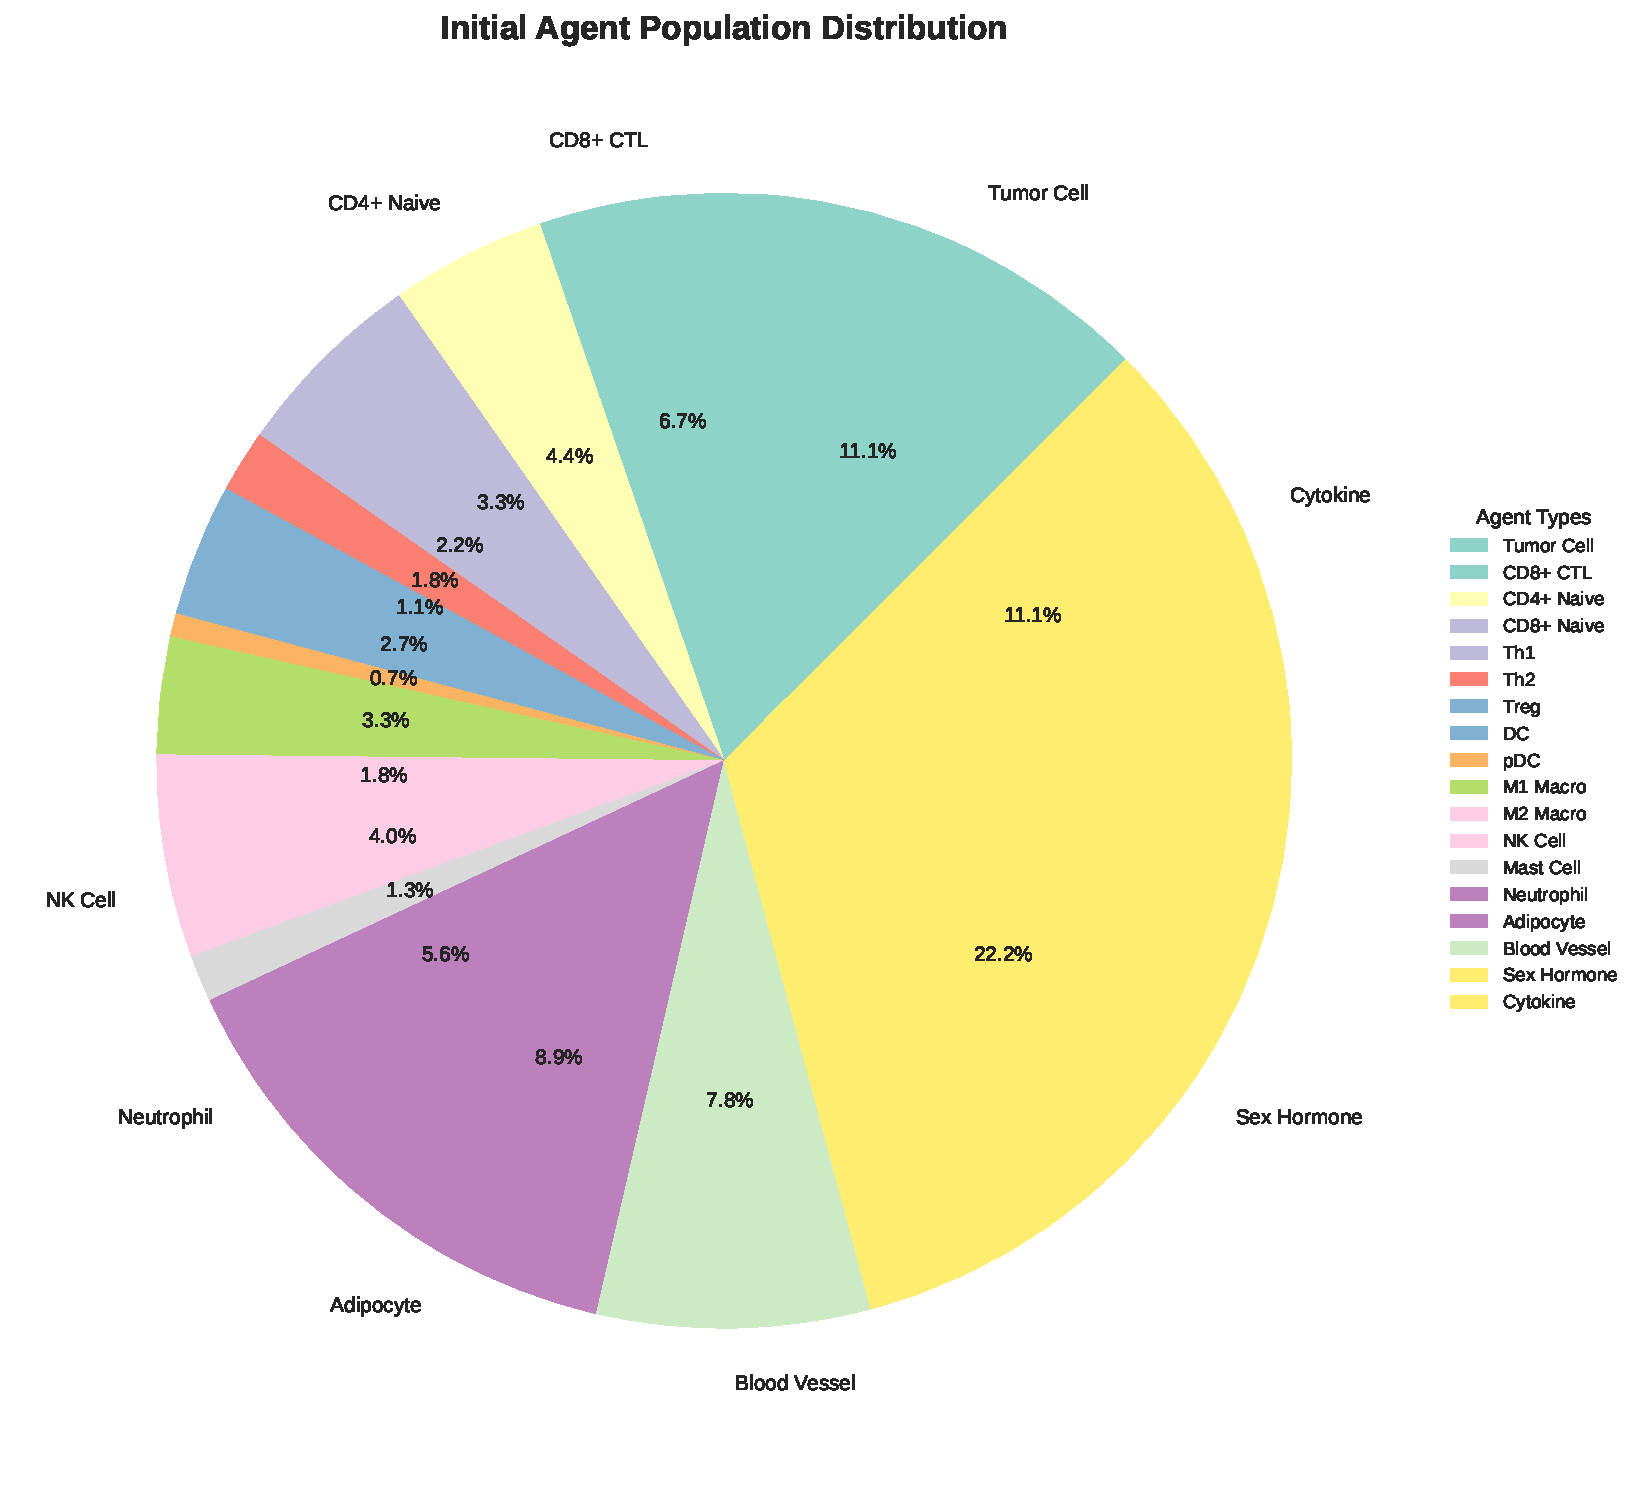
\includegraphics[width=0.8\textwidth]{figures/agent_population_pie.pdf}
\caption{Initial distribution of the 18 agent types in a typical RCC simulation. The model captures the complex cellular ecology of the tumor microenvironment, from tumor cells and diverse immune populations to supporting stromal elements and signaling molecules. Each agent type follows its own behavioral rules, yet their interactions generate emergent system-level dynamics that determine treatment outcomes.}
\label{fig:agent_population}
\end{figure}

\subsection{The Repast4Py Advantage: Scaling Up Without Giving Up}

Modeling individual cells is computationally expensive. A realistic tumor contains millions of cells, each interacting with its neighbors at every time step. Traditional single-process frameworks like Mesa \cite{mesa} hit scaling walls quickly. Our choice of Repast4Py \cite{repast4py} represents a fundamental architectural decision: we refuse to compromise biological realism for computational convenience.

Repast4Py's MPI-based parallel architecture distributes the computational load across multiple processors, allowing us to model larger tumor volumes with greater biological detail. More importantly, it provides a foundation for future scaling—as computational power increases, our model can grow with it, potentially reaching the million-cell simulations needed to capture full tumor complexity.

\begin{figure}[H]
\centering
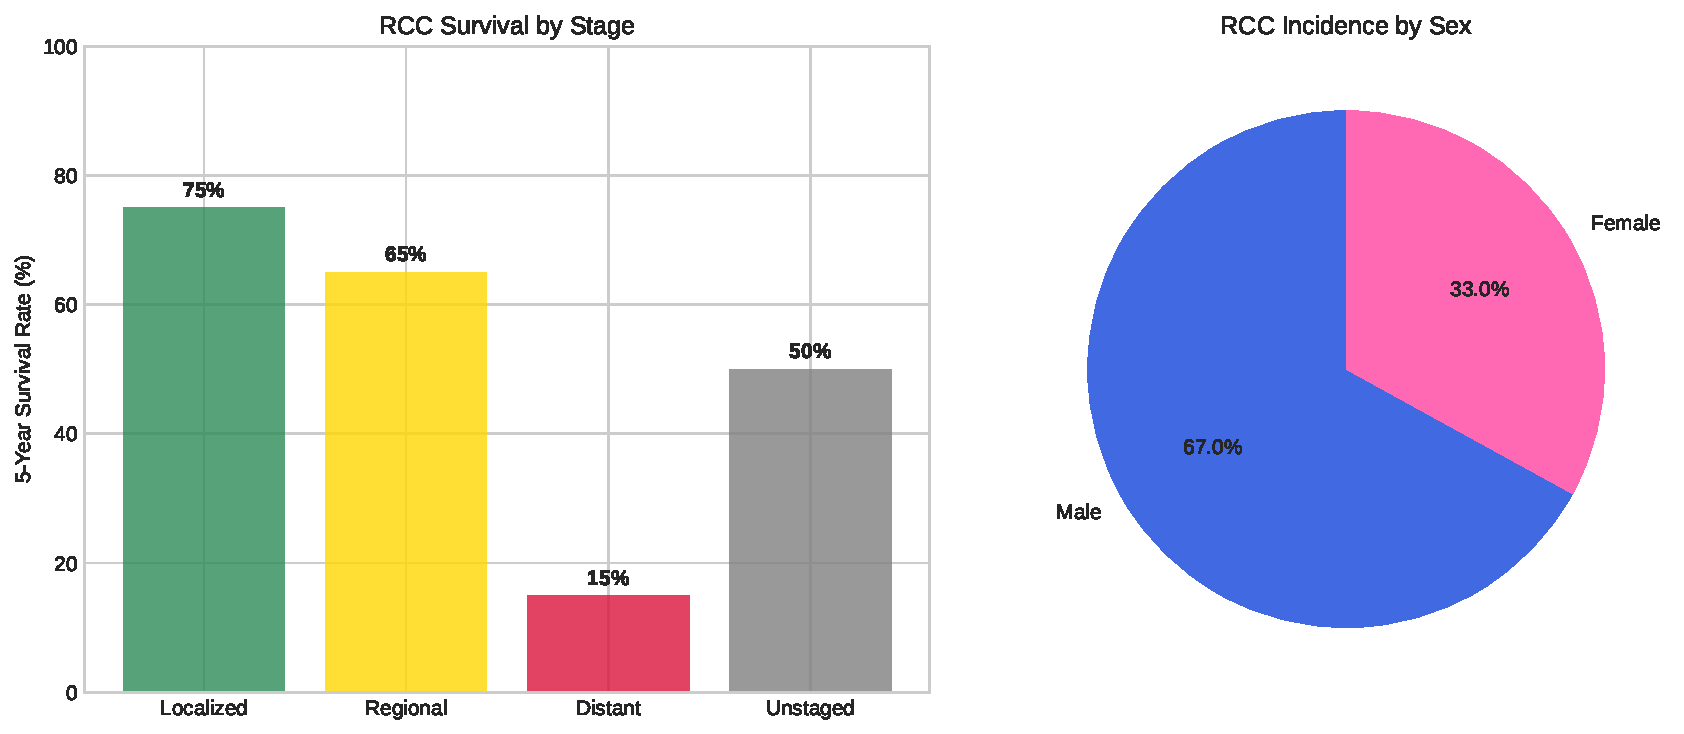
\includegraphics[width=0.9\textwidth]{figures/rcc_epidemiology.pdf}
\caption{The clinical reality driving our modeling efforts. \textbf{Left:} RCC survival rates vary dramatically by stage, with metastatic disease carrying a devastating 15\% five-year survival rate. \textbf{Right:} The pronounced male predominance in RCC incidence (2:1 ratio) reflects complex interactions between sex hormones and immune function that our model explicitly captures and explores.}
\label{fig:rcc_epidemiology}
\end{figure}

\section{Mission: Four Breakthroughs to Transform RCC Modeling}
\label{sec:intro_objectives}

This project represents more than an incremental improvement—it's a fundamental reimagining of how we model kidney cancer. Four interconnected objectives drive this transformation, each addressing critical limitations in current computational cancer research.

\subsection{Objective 1: Breaking the Single-Processor Ceiling}

The original Mesa-based RCC model was scientifically innovative but computationally constrained. Limited to single-processor execution, it could simulate only small tumor fragments—interesting for proof-of-concept, insufficient for clinical relevance.

\textbf{The Challenge:} Porting to Repast4Py isn't just changing frameworks—it's rebuilding the entire computational architecture. Agent hierarchies must be restructured, spatial indexing redesigned, and interaction logic adapted to handle distributed memory and inter-process communication.

\textbf{The Breakthrough:} MPI-based parallelism that scales with available computational resources. What once took hours on a single core can now run in minutes across multiple processors. More importantly, we've built a foundation that can grow—as tumors get larger and models get more detailed, the computational architecture can expand to meet the challenge.

\subsection{Objective 2: Adding the Missing Metabolic Layer}

Cancer cells don't exist in a vacuum—they compete fiercely for nutrients, creating metabolic gradients that shape the entire tumor ecosystem. Yet most computational cancer models ignore this fundamental biological reality.

\textbf{The Innovation:} We overlay a continuous 3D glucose concentration field on our discrete agent grid. Blood vessels inject glucose, which diffuses through tissue following Fick's laws. Tumor cells consume glucose at the dramatically elevated rates characteristic of the Warburg effect, creating depletion zones that impair immune function.

\begin{tcolorbox}[colback=glucose!10, colframe=glucose!50, title=\textbf{Metabolic Competition in Action}]
Imagine a cytotoxic T cell hunting tumor cells. As it approaches a large tumor mass, glucose levels drop. The T cell's killing capacity diminishes—not because of immune evasion, but because it lacks the metabolic fuel needed for its effector functions. This is the kind of emergent behavior that only becomes visible when metabolism is explicitly modeled.
\end{tcolorbox}

This metabolic layer introduces 8 new parameters governing glucose dynamics and adds chemotaxis—immune cells can follow glucose gradients when hunting for targets, providing a biologically plausible navigation mechanism.

\subsection{Objective 3: Validation Against Real-World Clinical Data}

Too many computational biology models live in academic isolation, validated against other models rather than clinical reality. We take a different approach: direct calibration against the ARON-1 clinical trial.

\textbf{The Standard:} ARON-1 provides sex-stratified treatment response data for ICI, TKI, and combination therapies—exactly the clinical scenarios our model is designed to predict. Every simulation parameter, every agent behavior, every treatment effect must ultimately pass this test: does it help explain real patient outcomes?

\textbf{The Process:} Systematic comparison of simulated vs. observed tumor growth trajectories, immune cell population dynamics, and treatment responses. Special attention to sex-specific differences that reflect the hormonal mechanisms explicitly modeled in our system.

\subsection{Objective 4: Intelligent Parameter Optimization}

With hundreds of parameters governing agent behaviors, manual calibration is hopeless. We implement Bayesian optimization using Optuna \cite{optuna}—an intelligent search strategy that learns from each simulation to guide the exploration of parameter space.

\textbf{The Strategy:} Rather than random parameter sampling, Bayesian optimization builds a probabilistic model of how parameter changes affect simulation outcomes. It focuses computational effort on promising regions of parameter space, efficiently converging on configurations that best reproduce clinical observations.

\textbf{The Goal:} A fully calibrated model where every parameter value is justified by its contribution to clinical accuracy. This isn't just about fitting data—it's about building confidence that the model captures real biological mechanisms.

\section{Journey Through the Cellular Universe: Report Roadmap}
\label{sec:intro_structure}

This report takes you on a journey from biological theory to computational implementation to clinical validation. Each chapter builds on the previous ones, constructing a complete picture of how individual cellular decisions aggregate into patient outcomes.

\textbf{Chapter 2: Theoretical Foundations} sets the stage by exploring the biological and mathematical principles underlying our approach. We compare agent-based modeling with traditional equation-based approaches, dive deep into RCC immunology, and examine the metabolic dynamics that shape tumor-immune interactions.

\textbf{Chapter 3: The Model Architecture} pulls back the curtain on our virtual tumor. You'll meet the 18 agent types, understand their interaction rules, and see how individual cell behaviors generate emergent population dynamics.

\textbf{Chapter 4: The Glucose Microenvironment} introduces the metabolic layer that sets our model apart. We'll explore how glucose gradients create invisible barriers to immune function and how tumor cells exploit metabolic competition.

\textbf{Chapter 5: DNA and Cellular Evolution} reveals how our 16-gene mutation system drives tumor heterogeneity and immune escape. Each tumor cell carries its own genetic story, determining its capabilities and vulnerabilities.

\textbf{Chapter 6: Treatment Systems} examines how ICI and TKI therapies work at the cellular level, and why combination treatments can achieve synergies that neither alone can provide.

\textbf{Chapter 7: Sex Hormones and Immune Modulation} explores the hormonal landscape that makes male and female patients respond differently to the same treatments.

\textbf{Chapter 8: Implementation Deep Dive} takes you under the hood of the computational architecture. From MPI parallelism to spatial indexing, this is where biological vision meets engineering reality.

\textbf{Chapter 9: The Parameter Universe} catalogs the hundreds of parameters that govern agent behavior, showing how biological knowledge translates into computational variables.

\textbf{Chapter 10: Results That Matter} presents the validation against ARON-1 clinical data, showing where the model succeeds, where it struggles, and what these results mean for future cancer research.

\textbf{Chapter 11: Looking Forward} concludes with lessons learned and the path ahead—how this work opens new possibilities for personalized cancer treatment.

Each chapter includes multiple visualizations, from conceptual diagrams to data plots, designed to make complex biological and computational concepts accessible and memorable. This isn't just a technical report—it's a story of how computational biology can transform our understanding of cancer and ultimately help save lives.

\vspace{2em}

\begin{chaptersum}
This chapter establishes the critical need for computational cancer modeling by highlighting three key insights: (1) the devastating clinical reality of metastatic kidney cancer with its 15\% five-year survival rate, (2) the profound but poorly understood role of sex hormones in determining treatment outcomes, and (3) the unique potential of agent-based modeling to capture the complex cellular dynamics that drive patient responses. Our approach represents a paradigm shift from population-based averages to individual patient prediction through virtual experimentation.
\end{chaptersum}
